\documentclass{cours}
\usepackage{esvect}
\usepackage{pgfplots}
\usepackage{multicol}
\usepackage{mathrsfs}
\usepackage{amssymb}
\usepackage{tikz-3dplot}
\usepackage{xr}
\usepackage{fontawesome}
\usetikzlibrary {decorations.text, backgrounds, intersections, patterns}

\begin{document}

\newcommand{\cc}{\ensuremath{\mathscr{C}}}

\setcounter{chapter}{26}
\chapter{Circuit mobile dans un champ magnétique stationnaire}
\section{Conversion de puissance mécanique en puissance électrique}%
\label{sec:conversion_de_puissance_mecanique_en_puissance_electrique}

\subsection{Rails de Laplace}%
\label{sub:rails_de_laplace}

On considère l'expérience des rails de Laplace, mais cette fois, il n'y a pas de générateur qui impose un courant dans le circuit, c'est une force extérieure $\vv*{F}{\text{ext}}$ qui met la barre en mouvement.

 \begin{center}
   
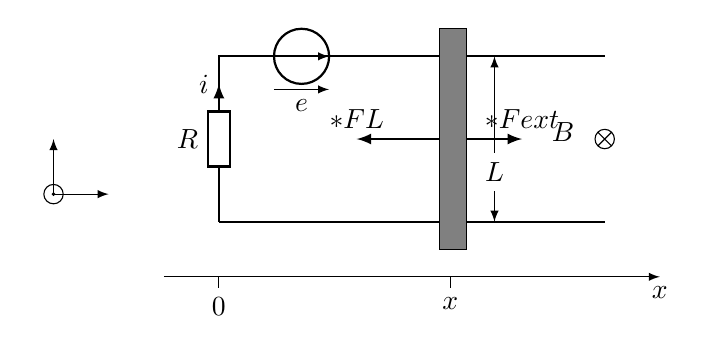
\begin{tikzpicture}[scale=0.7]
%tikz magnetisme
\coordinate (A) at (-1, 0.5);
\draw[-latex] (A) -- ++(1,0) node[right]{$\vex $} ;
\draw[-latex] (A) -- ++(0,1) node[left]{$\vey $} ;
\fill (A) circle(1pt);
\draw (A) circle(5pt);
\draw (A) ++ (-135:5pt) node[below left]{$\vez $}; 

\coordinate (B) at (2,0);
  \draw[thick] (B) -- ++(0, 1) ++(0,1) -- ++(0,1) -- ++(7, 0)
  (B) -- ++(7,0)
(B) ++ (-0.2,1) rectangle ++(0.4, 1);
\draw (B) ++(-0.2, 1.5) node[left] {$R$};
\draw[thick] (3.5, 3) circle(0.5);
\draw[-latex] (3, 3) -- ++(1,0);
\draw[-latex] (3, 2.4) -- ++(1,0) node[below, midway ]{$e$};

\draw[thick, -latex] (B) ++ (4, 1.5) coordinate (C) -- ++(1.5,0) node[above]{$\vv*{F}{\text{ext}}$};  
\draw[thick, -latex] (C) -- ++ (-1.5, 0) node[above]{$\vv*{F}{L}$};

  \draw[fill=gray] (B) ++(4,-0.5) rectangle ++(0.5, 4);
  \draw[latex-latex] (B) ++(5, 0) --  ++(0,3) node[pos=0.3,fill=white]{$L$};
  \draw[thick, -latex] (B) ++(0,2) -- ++(0,0.5) node[left]{$i$ };
  \draw (B) ++(7,1.5) circle (5pt)
  +(45:5pt) -- +(-135:5pt)
+(-45:5pt) -- +(135:5pt)
  node[left, xshift=-5pt]{$\vv{B}$};
  \draw[-latex] (1, -1) -- (10, -1) node[below]{$x$};
  \draw (2,-1) -- ++ (0, -0.2) node[below]{$0$ };
  \draw (6.2,-1) -- ++ (0, -0.2) node[below]{$x$ };
\end{tikzpicture}
\captionof{figure}{Expérience des rails de Laplace dans laquelle un opérateur applique une force à la barre pour la mettre en mouvement.}
 \end{center}

On note $\vv{v}= v \vex = v \dt{x}$ la vitesse de la barre. Le flux du champ magnétique à travers le circuit est 
\begin{equation}
  \Phi = BLx
\end{equation}

Comme $x$  varie au cours du temps, le flux du champ magnétique varie et il y a une fem $e$ induite dans le circuit. On a 
\begin{equation}
  e = -\dt{\Phi} = - BL \dt{x} = -BLv
\end{equation}  

Dans ces conditions, on peut écrire la puissance dissipée par effet Joule comme 
\begin{equation}
  P_\text{Joule} = ei = \frac{e^2}{R} = \frac{(BLv)^2}{R}\, .
\end{equation}

La puissance fournie par la force extérieure est 
\begin{equation}
  P_\text{ext} = \vv*{F}{\text{ext}}\cdot \vv{v}
\end{equation}
Comme on suppose que la barre avance à vitesse constante, le principe fondamental de la dynamique permet d'écrire que la somme des forces appliquées est nulle, et donc 
\begin{equation}
  F_\text{e} = -F_L = -iLB \vex  = -\frac{e}{R}LB \vex  = \frac{B^2L^2v}{R} \vex 
\end{equation}
La puissance fournie par $\vv*{F}{\text{ext}}$ est donc 
\begin{equation}
  P_\text{ext} = \vv*{F}{\text{ext}}\cdot\vv{v} = \frac{(BLv)^2}{R} = P_{\text{Joule}}.
\end{equation}

On a montré que la puissance mécanique fournie par l'opérateur qui tire sur la barre est convertie en une puissance électrique dissipée par effet Joule dans la résistance. Il y a conversion de puissance mécanique en puissance électrique. 

\subsection{Spire en rotation}%
\label{sub:spire_en_rotation}

On reprend l'exemple de la spire rectangulaire en rotation autour d'une axe fixe, plongée dans un champ magnétique uniforme et stationnaire.

\begin{center}
\tdplotsetmaincoords{70}{40}
  \begin{tikzpicture}[tdplot_main_coords]
  \tikzset{axe/.style={-latex, thick, gray}}
  \draw[axe] (-1,0,0) -- (7,0,0) node[right, color=black]{$x$};
  \draw[axe] (0,-3,0) -- (0,3,0) node[above, color=black]{$y$};
  \draw[axe] (0,0,-3) -- (0,0,3) node[above, color=black]{$z$};
  \draw[tdplot_main_coords](0,0,0) node[left]{$O$ };
  \tdplotsetrotatedcoords{90}{-45}{0}
  \draw[line width=3pt, white, tdplot_rotated_coords](-2, 0, 0) -- (-2, -4, 0);
  \draw[thick, tdplot_rotated_coords](-2,0,0)  node[below left](A){$A$}-- (2, 0, 0)  node[above left](D){$D$}-- (2, -6, 0) node[above right](C){$C$}  -- (-2, -6, 0) node[below](B){$B$}  -- cycle;
  \draw[thick, fill=white, tdplot_rotated_coords] (1.7, -2, 0) -- (1.7, -4, 0) -- (2.3, -4, 0) --  (2.3,-2, 0) node[midway, above, sloped]{$R$} -- cycle;  
  \draw[latex-latex] (A.east) -- node[fill=white, inner sep=2pt]{$\ell$} (B.west);
  \draw[latex-latex, tdplot_rotated_coords] (-2, -6.5, 0) -- node[pos=0.3,fill=white, inner sep=2pt]{$L$} (2, -6.5, 0);
  \draw[thick, tdplot_rotated_coords, -latex] (0, 0, 0) -- (-1, 0, 0) node[left]{$i$}; 
  \draw[tdplot_main_coords, -latex, thick] (9, 0, 0) -- ++(0,0, 1) node[midway, right]{$\vv{B} = B \vez $ }; 
   \tdplotsetthetaplanecoords{90}
   \tdplotdrawarc[tdplot_rotated_coords, -latex]{(0,0,0)}{1.5}{90}{45}{right}{$\theta$};
  \end{tikzpicture}
\captionof{figure}{Spire rectangulaire mise en rotation autour d'un axe fixe dans un champ magnétique extérieur stationnaire et uniforme.}
\end{center}
on procède exactement de la même manière que pour le cas précédent, sauf que cette fois on applique un couple $\Gamma_{\text{ext}}$ par rapport à l'axe $x$ à la spire, ce qui la met en rotation à vitesse angulaire $\omega = \dot{\theta}$ constante.

La puissance mécanique fournie à la spire est
\begin{equation}
  P_\text{meca} = \Gamma_{\text{ext}}\omega\, .
\end{equation}
Le flux du champ magnétique à travers le circuit est 
\begin{equation}
  \Phi = BS\cos(\theta)\, ,
\end{equation}
et donc la force électromotrice induite est 
\begin{equation}
  e = BS\omega\sin(\theta)
\end{equation}
L'intensité du courant électrique qui circule dans la spire est $i=\frac{e}{R}$. Et donc la spire subit couple du aux forces de Laplace qui vaut
\begin{equation}
  \Gamma_\text{Laplace} = \vv{\mu} \wedge \vv{B} \cdot \vex  = -iBS\sin(\theta)  
\end{equation}
Comme la spire tourne à vitesse constante dans le référentiel d'étude que l'on suppose galiléen, on peut écrire (TMC) $\Gamma_{ext} = -\Gamma_{\text{Laplace}}$, et la puissance mécanique devient
\begin{equation}
  P_\text{meca} = iBS\omega\sin(\theta) = \frac{e}{R}BS\omega\sin(\theta) = \frac{(BS\omega\sin(\theta))^2}{R}
\end{equation}

La puissance électrique dissipée par effet Joule dans la résistance est 
\begin{equation}
  P_\text{Joule}= Ri^2 = \frac{e^2}{R}=\frac{(BS\omega\sin(\theta))^2}{R} = P_\text{meca}
\end{equation}
On retrouve à nouveau que l'intégralité de la puissance mécanique fournie à la spire est convertie en puissance électrique dissipée par effet Joule dans la spire.

\subsection{Freinage par induction}%
\label{sub:freinage_par_induction}

Lorsqu'un conducteur électrique est en mouvement dans un champ magnétique non uniforme, la variation du flux du champ magnétique à travers une partie du conducteur va induire des courants électriques appelés \textbf{courants de Foucault} à l'intérieur du conducteur. 

À cause de ces courants induits, le conducteur subira une force de Laplace qui va le freiner. Le fait que la force freine le conducteur est une application directe de la loi de modération de Lenz : c'est le mouvement du conducteur qui produit les courants induits, donc l'effet de ces courants doit être de diminuer le mouvement du conducteur.

Nous allons établir l'expression du la force de freinage sur un cas modèle simple. On considère que le conducteur est une spire rectangulaire de largeur $L$ qui se déplace à la vitesse $\vv{v}=v \vex $. Dans la zone $x<0$ le champ magnétique extérieur est nul et dans la zone $x>0$, on a $\vv{B}=B \vez $.
\begin{center}
  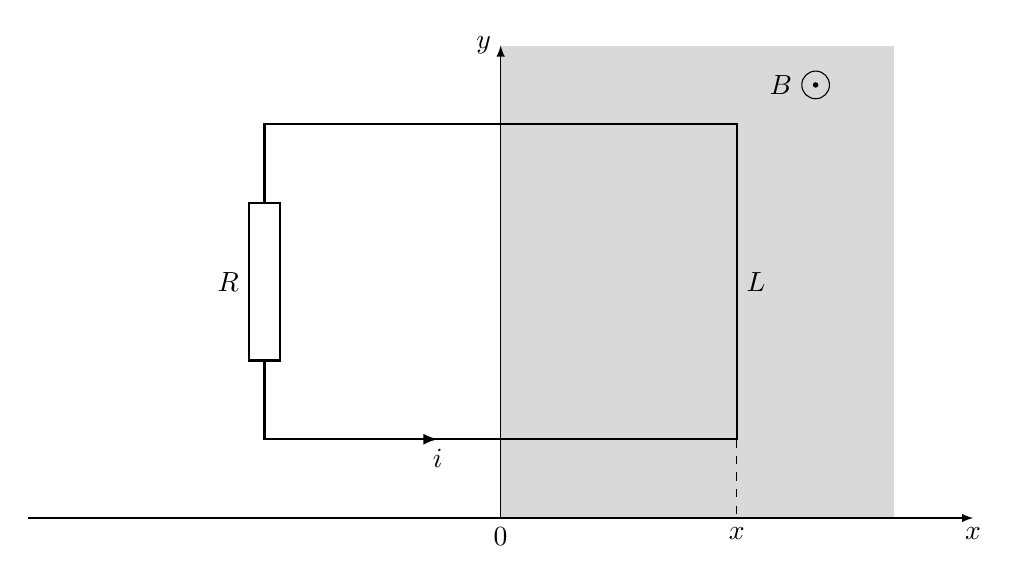
\begin{tikzpicture}
   \fill[gray!30] (0, -3) rectangle (5,3);
   \draw[-latex] (0, -3) node[below]{$0$} -- (0,3) node[left]{$y$};
   \draw[-latex] (-6, -3) -- (6,-3) node[below]{$x$};
  \draw (4, 2.5) circle (5pt) node[left, xshift=-5pt]{$\vv{B}$};
  \fill (4,2.5) circle(1pt);
  \draw[thick] (-3, -2) rectangle (3, 2);
  \draw (3, 0) node[right] {$L$};
  \draw[dashed](3, -2) -- (3, -3) node[below]{$x$};
  \draw[thick, -latex] (-1, -2) -- ++(0.2, 0) node[below]{$i$};
  \draw[thick, fill=white] (-3.2, -1) rectangle (-2.8, 1); 
  \draw (-3.2, 0) node[left]{$R$};
  \end{tikzpicture}
\end{center}
La force électromotrice induite dans la spire est 
\begin{equation}
  e = -\dt{\Phi} = -\dt{BLx} = -Blv \, ,
\end{equation} 
et le courant induit dans la spire est
\begin{equation}
  i = \frac{e}{R} = -\frac{Blv}{R} 
\end{equation}
La force de Laplace subie par la spire s'exerce uniquement sur la portion de la spire dirigée suivant $\vey$ dans la zone de champ, car les forces de Laplace qui s'exercent sur les portions suivant $\vex$ se compensent. On trouve que la force de Laplace subie par la spire est
\begin{equation}
  \vv*{F}{\text{Laplace}} = iLB\vex = -\frac{B^2L^2}{R}v \vex = -\frac{B^2L^2}{R}\vv{v} = -k\vv{v} \quad \text{avec} \quad k\geq 0
\end{equation}
Il s'agit donc bien d'une force de freinage (car opposée à $\vv{v}$. On remarque également que la force est proportionnelle à la vitesse de la spire, c'est une force qui ressemble beaucoup à une force de frottement fluide.

Le freinage par induction est utilisé entre autres pour ralentir les poids lourds dans les descentes. L'avantage de ce système est que contrairement au freinage par friction, il l'y a pas d'usure mécanique des freins qui peut être une source de leur défaillance.

\section{Conversion de puissance électrique en puissance mécanique : le haut-parleur électrodynamique}%
\label{sec:conversion_de_puissance_electrique_en_puissance_mecanique_le_haut_parleur_electrodynamique}

On a déjà vu que les forces de Laplace permettent de convertir de la puissance électrique en puissance mécanique. Dans l'expérience des rails de Laplace, on a déjà montré que la puissance mécanique reçue par la barre est égale à :
\begin{equation}
  P_\text{Laplace} = i \dt{\Phi} = -ie = P_G\, ,
\end{equation}
où $P_G$ est la puissance fournie par le générateur. On montre donc que la puissance mécanique reçue par la barre est égale à la puissance électrique fournie par le générateur. Il y a conversion de puissance électrique en puissance mécanique.

\begin{center}
  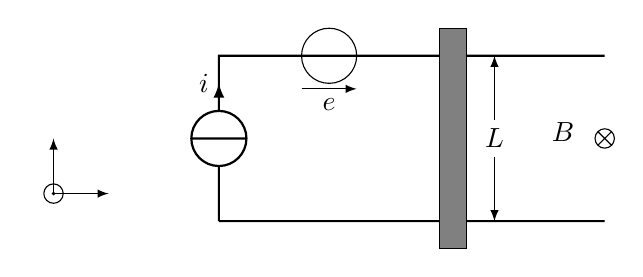
\begin{tikzpicture}[scale=0.7]
  %tikz magnetisme
    \coordinate (A) at (-1, 0.5);
    \draw[-latex] (A) -- ++(1,0) node[right]{$\vex $} ;
    \draw[-latex] (A) -- ++(0,1) node[left]{$\vey $} ;
    \fill (A) circle(1pt);
    \draw (A) circle(5pt);
    \draw (A) ++ (-135:5pt) node[below left]{$\vez $}; 
    
    \coordinate (B) at (2,0);
    \draw[thick] (B) -- ++(0, 1) ++(0,1) -- ++(0,1) -- ++(7, 0)
                 (B) -- ++(7,0)
                 (B) ++ (0,1.5) circle(0.5)
                 (B) ++(-0.5, 1.5) -- ++(1,0);
    \draw[fill=gray] (B) ++(4,-0.5) rectangle ++(0.5, 4);
    \draw[latex-latex] (B) ++(5, 0) -- node[fill=white]{$L$ } ++(0,3);
    \draw[thick, -latex] (B) ++(0,2) -- ++(0,0.5) node[left]{$i$ };
    \draw (B) ++(7,1.5) circle (5pt)
          +(45:5pt) -- +(-135:5pt)
          +(-45:5pt) -- +(135:5pt)
          node[left, xshift=-5pt]{$\vv{B}$};
    \draw (B) ++(2, 3) circle (0.5);
    \draw[-latex] (B) ++(1.5, 2.4) -- ++(1,0) node[midway, below]{$e$};
  \end{tikzpicture}
  \captionof{figure}{Conversion de puissance électrique en puissance mécanique dans l'expérience des rails de Laplace.}
\end{center}

La conversion de puissance électrique en puissance mécanique intervient principalement dans les différents moteurs électriques (moteur à courant continu, moteur synchrone, moteur asynchrone) mais aussi dans les haut-parleurs électrodynamiques. On montre ci-dessous le schéma d'un haut-parleur. On fait passer un courant dans une bobine située dans une zone de champ magnétique créé par un aimant permanent. La force de Laplace subie par la bobine provoque son déplacement et ainsi le déplacement de la membrane à laquelle elle est attachée. 

Un courant variable permet de faire vibrer la membrane qui transmet ces vibrations à l'air et produit un son.

\begin{center}
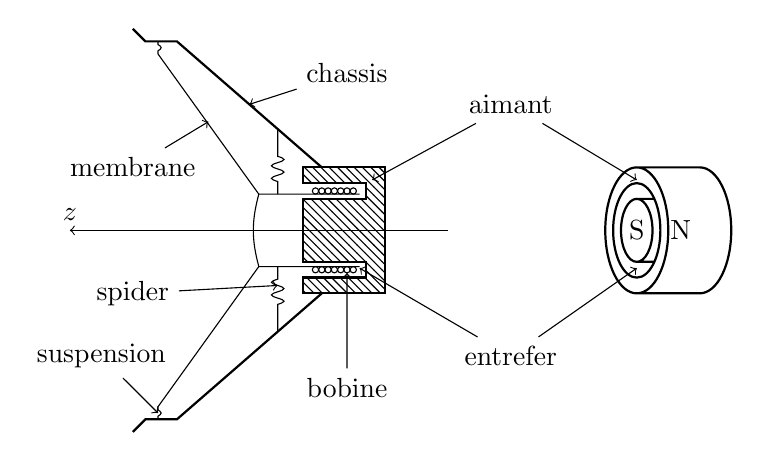
\begin{tikzpicture}[scale=0.8]
  \draw[thin,<-] (-1,0) node[above] {$z$} -- (5,0);
  \draw[thick,name path=chassis] % Le chassis
      (0,3.2) -- (0.2,3) -- (0.7,3) -- (3,1)
      (0,-3.2) -- (0.2,-3) -- (0.7,-3) -- (3,-1);
  \draw[thick,pattern=north west lines] % L'aimant
      (2.7,1) -- (4,1) -- (4,-1) -- (2.7,-1) --
      (2.7,-0.75) -- (3.7,-0.75) -- (3.7,-0.5) -- (2.7,-0.5) --
      (2.7,0.5) -- (3.7,0.5) -- (3.7,0.75) -- (2.7,0.75) -- cycle;
  \draw % La membrane
      (0.4,3) -- (0.4,2.95) {[rotate=-90] sin ++(0.05,0.05) cos ++(0.05,-0.05)} -- (0.4,2.8)
          -- (2,0.575) coordinate (M1) -- (3.6,0.575)
      (0.4,-3) -- (0.4,-2.95) {[rotate=90] sin ++(0.05,-0.05) cos ++(0.05,0.05)} -- (0.4,-2.8)
          -- (2,-0.575) coordinate (M2) -- (3.6,-0.575)
      (M1) to[out=255,in=105] (M2);
  \foreach \x in {0,1,...,6} \draw  % La bobine
      (2.9,0.625) ++(0.\x,0) circle [radius=0.05]
      (2.9,-0.625) ++(0.\x,0) circle [radius=0.05];
  % Le spider
  \coordinate (S1) at ($(M1)+(0.3,0)$);
  \coordinate (S2) at ($(M2)+(0.3,0)$);
  \path[name path=spider] ($(S1)+(0,2)$) -- ($(S2)+(0,-2)$);
  \draw[name intersections={of=chassis and spider,sort by=spider}] % Le spider
      (S1) -- ++(0,0.2) {[rotate=90]
          sin ++(0.05,0.1) cos ++(0.05,-0.1) sin ++(0.05,-0.1) cos ++(0.05,0.1)
          sin ++(0.05,0.1) cos ++(0.05,-0.1) sin ++(0.05,-0.1) cos ++(0.05,0.1)
          } -- (intersection-1)
      (S2) -- ++(0,-0.2) {[rotate=-90]
          sin ++(0.05,-0.1) cos ++(0.05,0.1) sin ++(0.05,0.1) cos ++(0.05,-0.1)
          sin ++(0.05,-0.1) cos ++(0.05,0.1) sin ++(0.05,0.1) cos ++(0.05,-0.1)
          } -- (intersection-2)
      ;

  \startscope[shift={(8,0)},thick]
  \draw
      (0,0) ellipse [y radius=1, x radius=0.5]
      (0,1) -- (1,1) arc [y radius=1, x radius=0.5, start angle=90, end angle=-90]
      -- (0,-1);
  \draw[clip] (0,0) ellipse [y radius=0.75, x radius=0.375];
  \draw
      (0,0) ellipse [y radius=0.5, x radius=0.25]
      (0,0.5) -- +(1,0)
      (0,-0.5) -- +(1,0);
  \stopscope
  
  \node at (8.7,0) {N};
  \node at (8,0) {S};
  \node at (6,2) (aimant) {aimant};
  \draw[->] (aimant) -- (3.8,0.8);
  \draw[->] (aimant) -- (8,0.8);
  \node at (6,-2) (entrefer) {entrefer};
  \draw[->] (entrefer) -- (3.6,-0.6);
  \draw[->] (entrefer) -- (8,-0.6);
  \node at (3.4,-2.5) (bobine) {bobine};
  \draw[->] (bobine) -- (3.4,-0.675);
  \node at (3.4,2.5) (chassis) {chassis};
  \draw[->] (chassis) -- (1.85,2);
  \node at (0,1) (membrane) {membrane};
  \draw[->] (membrane) --(1.2,1.725);
  \node at (0,-1) (spider) {spider};
  \draw[->] (spider) -- ($(S2)+(0,-0.3)$);
  \node at (-0.5,-2) (suspension) {suspension};
  \draw[->] (suspension) -- (0.4,-2.9);
  
\end{tikzpicture}
\captionof{figure}{Schéma d'un haut-parleur électrodynamique.}
\end{center}

On peut modéliser le haut-parleur par une configuration de rails de Laplace dans laquelle la barre est attachée par un ressort à un support fixe comme sur le schéma ci-dessous.

\begin{center}
  
  \begin{tikzpicture}[scale=0.7]
  %tikz magnetisme
    \coordinate (A) at (-1, 0.5);
    \draw[-latex] (A) -- ++(1,0) node[right]{$\vex $} ;
    \draw[-latex] (A) -- ++(0,1) node[left]{$\vey $} ;
    \fill (A) circle(1pt);
    \draw (A) circle(5pt);
    \draw (A) ++ (-135:5pt) node[below left]{$\vez $}; 
    
    \coordinate (B) at (2,0);
    \draw[] (B) -- ++(0, 1) -- ++(0,2) to[L=$L$] ++(2,0) coordinate(fem) -- ++(5, 0)
                 (B) -- ++(7,0)
                 (B) ++ (0,1.5) circle(0.5)
                 (fem) ++(1, 0) circle (0.5);
    \draw[-latex] (fem) ++(0.5,0.7) -- ++(1,0) node[midway, above] {$e$ };
    \draw[-latex] (B) ++(-0.7, 1) -- ++(0,1) node[left, midway]{$u$ };
    \draw[fill=gray] (B) ++(4,-0.5)  coordinate(A) rectangle ++(0.5, 4);
    \draw[latex-latex] (B) ++(5, 0) -- node[fill=white]{$\ell$ } ++(0,3);
    \draw[ -latex] (B) ++(0,2) -- ++(0,0.5) node[left]{$i$ };
    \draw (B) ++(7,1.5) circle (5pt)
          +(45:5pt) -- +(-135:5pt)
          +(-45:5pt) -- +(135:5pt)
          node[left, xshift=-5pt]{$\vv{B}$};
    \draw[fill=gray] (B) ++(1, 0.5) rectangle ++(0.5, 2); 
    \draw[decorate, decoration={pre length=3mm, post length=3mm, zigzag}] (B) ++(1.5, 1.5) -- ++(2.5, 0) node[midway, above]{$k$ };
    \draw (B) ++(1.25, 0.5) -- ++(1, -2) -- ++(1,0) node[right]{Support fixe};
    \draw (A) ++(0.5, 1) -- ++(1, -1) -- ++(1,0) node[right]{Bobine attachée à la membrane};
  \end{tikzpicture}
  \captionof{figure}{Modélisation du haut-parleur par une configuration de rails de Laplace.}
\end{center}

Dans cette modélisation, l'inductance $L$ est l'inductance propre de la bobine du haut-parleur, la bobine est soumise à la force de Laplace
\begin{equation}
  \vv*{F}{L} = i\ell B \vex \, ,
\end{equation}
à la force de rappel du ressort
\begin{equation}
  \vv*{F}{r} = -kx \vex \, ,  
\end{equation}
et à une force de frottement fluide modélisant l'interaction de la bobine avec l'air
\begin{equation}
  \vv{f} = -h\vv{v}\, ,
\end{equation}
où $\vv{v} = \dot{x}\vex$  est la vitesse de la barre. Le principe fondamentale de la dynamique appliqué à la barre dans un référentiel galiléen, projeté sur l'axe $\vex $ donne
\begin{equation}
  m \ddot{x} = i\ell B -kx -h \dot{x}
  \label{eq:pfd}
\end{equation}

On a par ailleurs, l'équation électrique du circuit. On note $e$ la fem induite dans la bobine par le champ magnétique produit par l'aimant, on a 
\begin{equation}
  e = -\dt{\Phi} = -B\ell \dot{x}
\end{equation}
Et la loi des mailles donne 
\begin{equation}
  u = L \dt{i} -e = L \dt{i} + B \ell \dot{x} 
  \label{eq:elec}
\end{equation}

On peut multiplier l'équation~\ref{eq:pfd} par $-\dot{x} $, ajouter l'équation~\ref{eq:elec} multipliée par $i$ pour obtenir :
\begin{equation}
  -m \ddot{x} \dot{x} + ui  = -i\ell B \dot{x} + kx \dot{x} + h \dot{x}^2 + L \dt{i}i+i\ell B \dot{x}
\end{equation}
soit
\begin{equation}
  ui -h \dot{x}^2 = \dt{U}
\end{equation}
où
\begin{equation}
  U = \frac{1}{2} m \dot{x}^2 + \frac{1}{2}Li^2 + \frac{1}{2}k x^2  
\end{equation}
représente l'énergie totale du système. On montre ainsi que la variation d'énergie du système est égale à la différence entre la puissance reçue de la part du générateur ($ui$) et la puissance perdue par frottements fluides ($-h \dot{x}^2$).
\end{document}
